\documentclass[conference]{IEEEtran}
\IEEEoverridecommandlockouts
% The preceding line is only needed to identify funding in the first footnote. If that is unneeded, please comment it out.
\usepackage{algorithm}
\usepackage{cite}
\usepackage{amsmath,amssymb,amsfonts}
\usepackage{array,booktabs}
\usepackage{algorithmic}
\usepackage{graphicx}
\usepackage{textcomp}
\usepackage{caption}
\usepackage{subcaption}
\usepackage{stackrel}
\usepackage{breqn}
% \usepackage{isomath}
\usepackage{mathtools}
\usepackage{xcolor}
\usepackage[utf8]{inputenc}
\usepackage[english]{babel}
\usepackage{amsthm}
\theoremstyle{definition}
\newtheorem{definition}{Definition}[section]
\usepackage[a4paper, total={184mm,239mm}]{geometry}
\def\BibTeX{{\rm B\kern-.05em{\sc i\kern-.025em b}\kern-.08em
    T\kern-.1667em\lower.7ex\hbox{E}\kern-.125emX}}
\begin{document}

\title{Black Wolf Optimization: A Hybridized Self-Adaptive and Automated Computational Framework\\
% {\scriptsize \textsuperscript{*}Note: Sub-titles are not captured in Xplore and
% should not be used}
% \thanks{Identify applicable funding agency here. If none, delete this.}
}

% \author{\IEEEauthorblockN{Anand Ravishanakar\IEEEauthorrefmark{1},
% Santhi Natarajan\IEEEauthorrefmark{2} and
% Bharathi Malakreddy\IEEEauthorrefmark{3}}
% \IEEEauthorblockA{Department of Artificial Intelligence and Machine Learning,
% BMS Institute of Technology and Management\\
% Bangalore, India\\
% Email: \IEEEauthorrefmark{1}anandravishankar12@gmail.com,
% \IEEEauthorrefmark{2}santhi.natarajan@bmsit.in,
% \IEEEauthorrefmark{3}bharathi\_m@bmsit.in}}

% 
% \author{\IEEEauthorblockN{Anand Ravishanakar}
% \IEEEauthorblockA{\textit{Department of Artificial Intelligence and Machine Learning} \\
% \textit{BMS Institute of Technology and Management}\\
% Bangalore, India  \\
% 1by17ec016@bmsit.in}
% \and
% \IEEEauthorblockN{Santhi Natarajan}
% \IEEEauthorblockA{\textit{Department of Artificial Intelligence and Machine Learning} \\
% \textit{BMS Institute of Technology and Management}\\
% Bangalore, India  \\
% santhi.natarajan@bmsit.in}
% \and
% \IEEEauthorblockN{\hspace{8mm}Bharathi Malakreddy}
% \IEEEauthorblockA{\hspace{12mm}\textit{Department of Artificial Intelligence and Machine Learning} \\
% \textit{\hspace{12mm}BMS Institute of Technology and Management}\\
% \hspace{12mm}Bangalore, India  \\
% \hspace{12mm}bharathi\_m@bmsit.in}
% }

\maketitle

\begin{abstract}
% For the past couple of decades the increased interaction between researchers from fields of Evolutionary Computing, Genetic Algorithms, Swarm Intelligence, Evolutionary Programming among others, has reshaped the future of nature-based computational intelligence in a positive sense. Taking advantage of this fusion, we present a hybrid algorithm which uses the blend of these sciences and redefines the existing methodology for intelligence systems. 
Multiple algorithms have been developed and deployed successfully to solve problems in selective optimization domains. The set of heuristic randomized optimization algorithms, inspired by natural evolution, form a unique branch of Computational Intelligence tagged as Evolutionary Algorithms (EA). In this paper, we present Black Wolf Optimization (BWO), a competition-induced EA replicating faunal behaviour. BWO has boosted accuracy levels to 95-97\% for real-world oncological datasets, which is a significant improvement on the current accuracy levels of 75-87.5\%. BWO incurs overhead in terms of time and computational resources taken. We have overcome this pitfall by accelerating BWO on HPC platforms with multiple GPUs,  that delivered a markup performance improvement of up to 517x.
\end{abstract}

\begin{IEEEkeywords}
BWO, Multi-Objective Optimization, Computational Intelligence, Swarm Optimization, Evolutionary Algorithms, GPU acceleration.
\end{IEEEkeywords}

\section{Introduction}

\subsection{Nature Inspired Multi-Objective Models: An Overview}

The traditional search and optimization techniques for either single-objective or multi-objective functions employ a single candidate solution which is tweaked to find the sweet spot of the global optimum. Multi-objective Functions have a general the form described in Equation \ref{e1}. A single Multi-objective Function can be viewed as $\textit{M}$ single-objective functions \cite{chankong}, having $\textit{K}$ equality bounds and $\textit{J}$ inequality bounds. The $\textit{n}$ input vector components $\textit{x\textsubscript{i}}$ are also bounded within a lower $\textit{x\textsubscript{i}\textsuperscript{L}}$ and upper $\textit{x\textsubscript{i}\textsuperscript{U}}$ bound. 

{\scriptsize
    \begin{align}
    \label{e1}
    Maximize/Minimize:f\textsubscript{m}(x)& &  m = 1,2\dots,M \\
    constraints:g\textsubscript{j}(x) \ge 0& & j=1,2\dots,J \nonumber\\
    h\textsubscript{k}(x) = 0& & k=1,2\dots,K \nonumber\\
    x\textsubscript{i}\textsuperscript{L} \le x\textsubscript{i} \le x\textsubscript{i}\textsuperscript{U} && i = 1,2\dots,n.\nonumber 
    \end{align}
}%

Solving these objective functions using traditional, single-candidate, unguided methods such as dynamic programming or greedy search has been successful when problems have a strong mathematical representation. Recent research focuses on unorthodox approaches in nature-based computational intelligence, employing both heuristic and meta-heuristic techniques, that offer approximate solutions to truly multi-objective functions. Whilst heuristic algorithms provide an acceptable yet non-optimal solution, meta-heuristics take this to the next level by introducing a fluid design of generation and selection of a set of feasible candidate solutions.  

% 
% \begin{figure}[htbp]
% \centerline{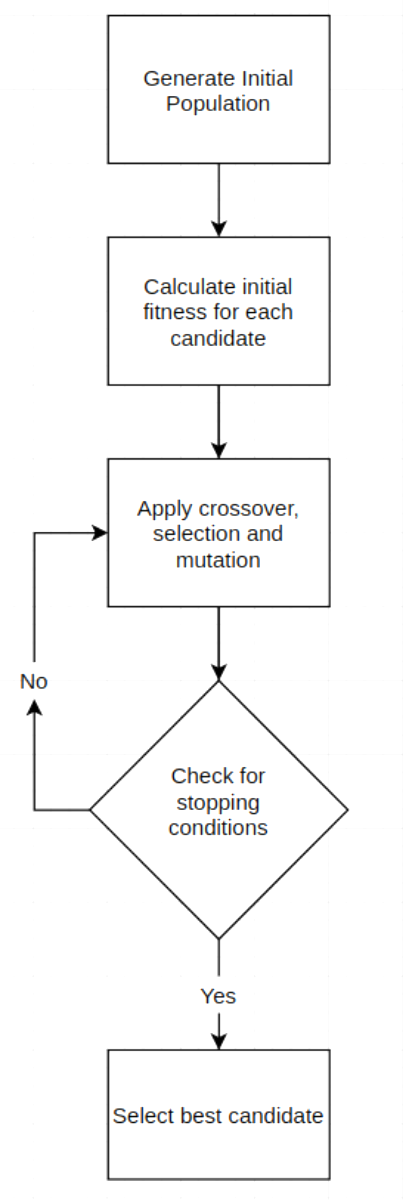
\includegraphics{ga.png}}
% \caption{Example of a figure caption.}
% \label{fig}
% % \end{figure}
% 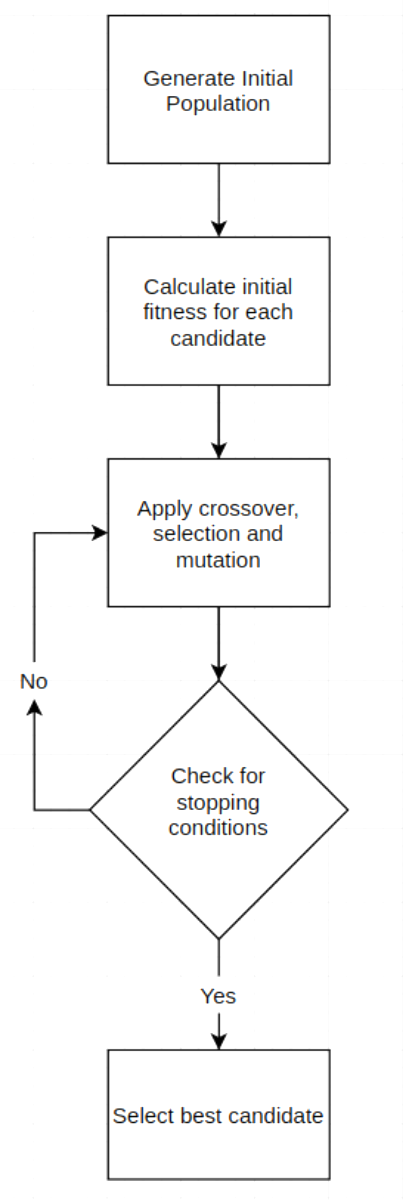
\includegraphics[width=4cm, height=4cm]{ga.png}
% 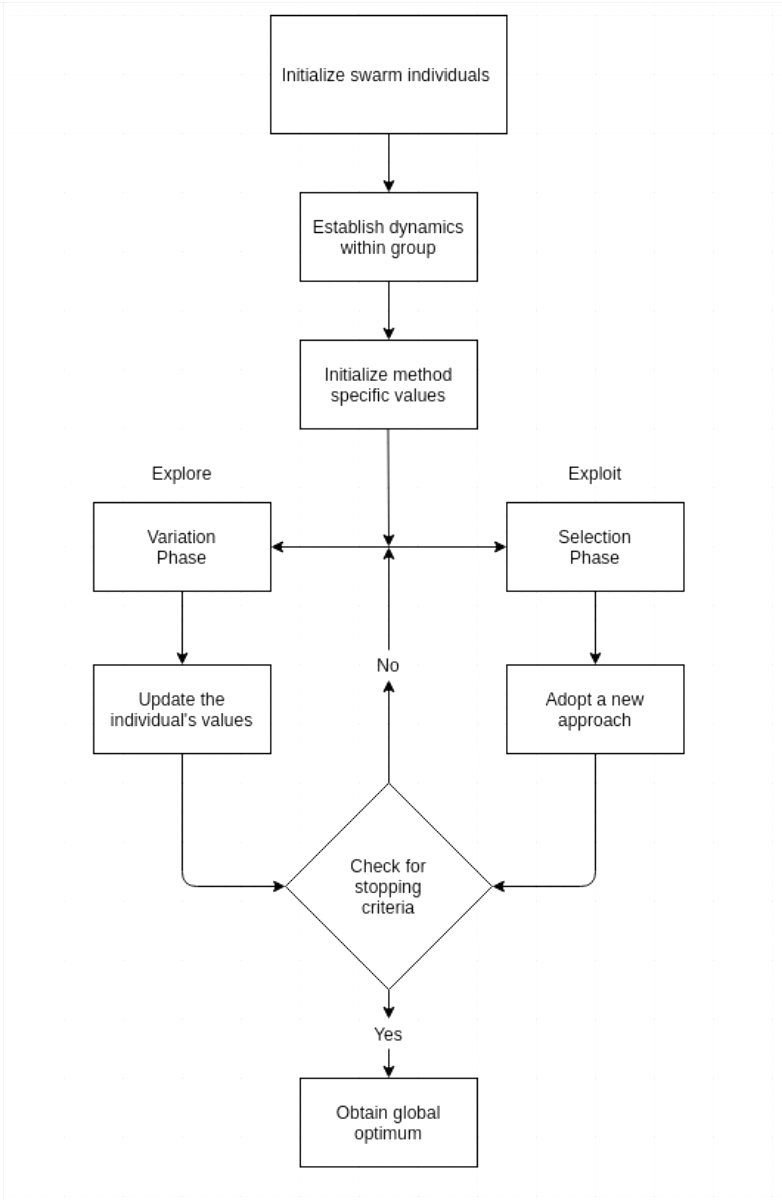
\includegraphics[width=6cm, height=6cm]{SI.png}
% \begin{figure}
% \centering
% \begin{subfigure}{5cm}
% \centering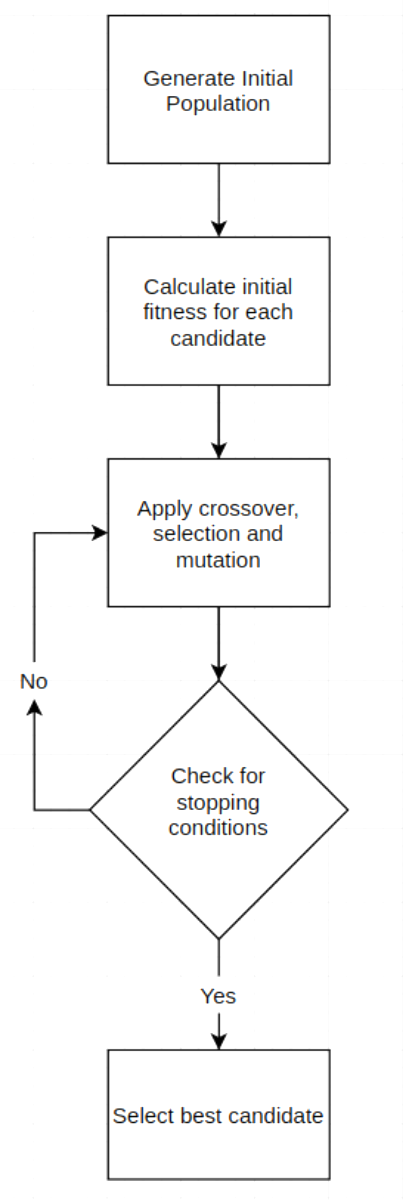
\includegraphics[height=8cm]{ga.png}
% \end{subfigure}%    
% \begin{subfigure}{5cm}
% \centering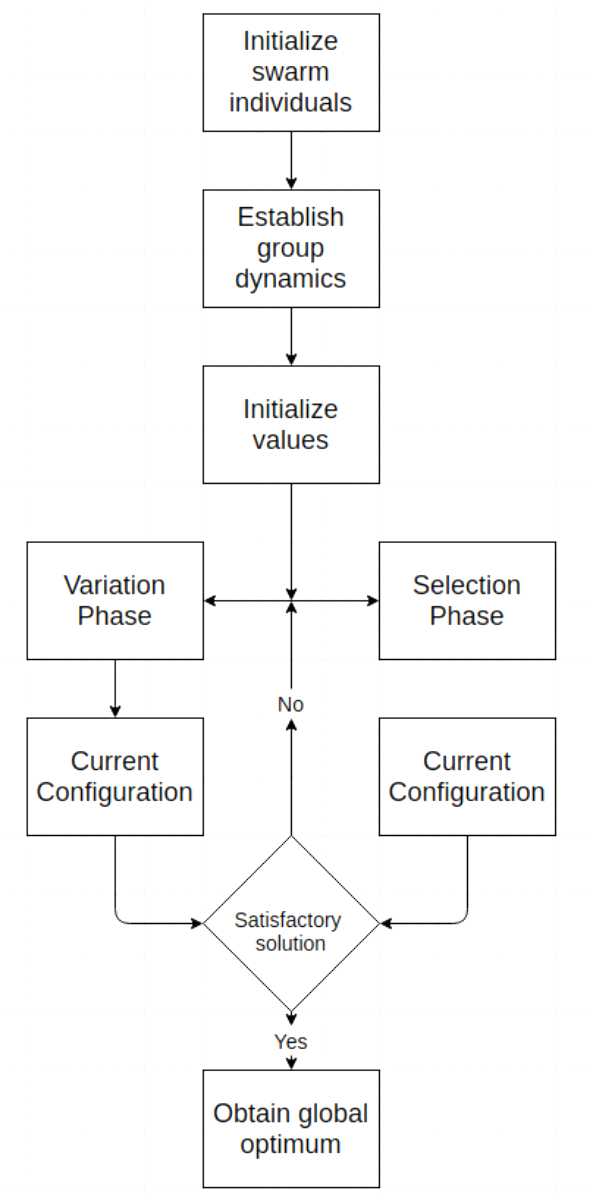
\includegraphics[height=8cm]{si.png}
% \end{subfigure}\vspace{8pt}
% \caption{GA and SI Flowcharts}
% \label{fig:flows}
% \end{figure}

\begin{figure}[t]
	\centering
	\begin{subfigure}{.16\textwidth}
		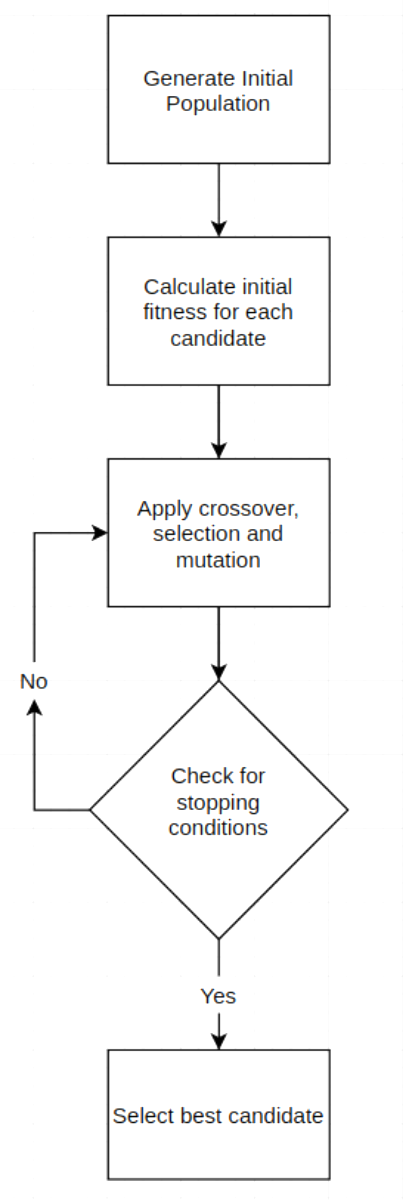
\includegraphics[width=\textwidth]{ga.png}
		
	\end{subfigure}
%%%%%%%%%%%%%%
%%%%%%%%%%%%%%
	\caption{Evolutionary Algorithms (EA)}
	\label{fig:comp}
\end{figure}
\vspace{-0.1cm}

Fig. $\ref{fig:comp}$ outlines the general flow of an EA. \cite{fried}. EA adopts the process of evolution and theory of natural selection to account for the survival and adaptability of candidate solutions. In algorithmic terms, an initial solution set is randomly seeded and based on fitness evaluator, ceratin solutions are discarded while new solutions are spwaned from the existing ones. This process continues till a sufficiently good solution is achieved. 

% SI models the collective interaction between the candidate solutions to self organize, share information amongst each other, and reach a common global optimum. 


\section{Existing Methodology}

\subsection{Base Learning Models}
Any existing machine learning framework involves a programmatic approach of tuning the internal hyperparameters for the desired outputs for a set of inputs. The most common technique used for selecting the best configuration is a grid search which involves trying out every possible configuration. An improvement in this is made in the form of random search which randomly chooses a configuration and rates it against a fitness function. 

Architectures like neural networks have an extensive set of hyperparameters making them extremely sensitive to their own configuration, as it affects the learning process. However, high-quality results cannot be guaranteed in a short time and inner tinkering cannot be performed as these networks function as black boxes. A general neural network architecture is shown in Algorithm $\ref{alg:nn}$ for $\textit{n}$ training examples in dataset $\textit{D}$. 

\begin{algorithm}[b]
\scriptsize
\caption{General Neural Network}
\label{alg:nn}
\begin{algorithmic}[1]
\STATE \textbf{Input:} D = \{(x\textsubscript{k}, y\textsubscript{k})\} $\forall$ k $\in$ (1, n), hyperparameter configuration = default
\WHILE{Stopping conditions are achieved}    
\STATE Evaluate y\textsubscript{k} based on input
\STATE Calculate $\delta$ i.e difference between \^y\textsubscript{k} and y\textsubscript{k}
\STATE Update weights according to hyperparameter configuration
\STATE Backpropogate the errors
\STATE Evaluate results against standard metrics
\ENDWHILE
\end{algorithmic}
\end{algorithm}


% 
% The most common form for a good search candidate for an ideal output vector $\vec{f\textsuperscript{0}}$ is given in Equation $\ref{eq:1}$ \cite{Osyczka}.
% 
% \begin{equation}
% \scriptsize
% \label{eq:1}
% f(\vec{x}) = \sum_{i=1}^{k}\frac{\vec{f\textsuperscript{0}} - f(\vec{x})}{\vec{f\textsuperscript{0}}}
% \end{equation}

Further improvements can be made by introducing dynamic programming models into the fold. The optimization problem is broken down into sub-problems and optimal solutions are found for them. The composition of these optimal sub-solutions results in an optimal global solution.  

\vspace{-0.2cm}




\begin{algorithm}[t]
\scriptsize
\caption{GWO}
\label{alg:gwo}
\begin{algorithmic}[1]
\STATE \textbf{Input:} Population size $\textit{n}$, random vectors $\vec{r\textsubscript{1}}$, $\vec{r\textsubscript{2}} \in$ [0,1], initial prey location $\vec{D}$, number of iterations \textit{I}, fitness function $\textit{f}$, coefficient vectors $\vec{A}$, $\vec{C}$ and $\vec{a}$
\STATE Set $\textit{t}$ = 0
\FOR{i $\in$ [1,n]}    
\STATE Generate wolf pack population $\textit{X\textsubscript{i}(t)}$ at instance $\textit{t}$
\STATE Evaluate each individual against the fitness function
\ENDFOR
\STATE Assign $\alpha, \beta, \delta$ titles to the top three solutions
\STATE Evaluate $\vec{D} = |\vec{C} \cdot \vec{X\textsubscript{p}}(t) - \vec{X}(t)|$
\FOR{\textit{i} in \textit{I}}
\FOR{Each individual in $\textit{n}$}  
\STATE $\vec{X\textsubscript{1}} = \vec{X\textsubscript{$\alpha$}} - \vec{A\textsubscript{1}} \cdot  \vec{D\textsubscript{$\alpha$}}$
\STATE $\vec{X\textsubscript{2}} = \vec{X\textsubscript{$\beta$}} - \vec{A\textsubscript{2}} \cdot  \vec{D\textsubscript{$\beta$}}$
\STATE $\vec{X\textsubscript{3}} = \vec{X\textsubscript{$\delta$}} - \vec{A\textsubscript{3}} \cdot  \vec{D\textsubscript{$\delta$}}$
\STATE Evaluate $\vec{X}(t+1) = \frac{\vec{X\textsubscript{1}} + \vec{X\textsubscript{2}} + \vec{X\textsubscript{3}}}{3}$
\ENDFOR
\STATE Update the coefficient vectors $\vec{A}$ and $\vec{C}$
\STATE $\vec{A} = 2\vec{a} \cdot \vec{r\textsubscript{1}} - \vec{a}$
\STATE $\vec{C} = 2\vec{r\textsubscript{2}}$
\STATE Linearly decrease $\vec{a}$ from 2 to 0
\STATE Update $\vec{X\textsubscript{$\alpha$}}, \vec{X\textsubscript{$\beta$}}, \vec{X\textsubscript{$\delta$}}$
\STATE Increment $\textit{t}$
\ENDFOR
\STATE $\vec{X\textsubscript{$\alpha$}}$ corresponds to the global optimum. 
\end{algorithmic}
\end{algorithm}

\begin{table}[!t]
\caption{\textsc{Previous Works on GWO}}
\label{table:pgwo}
\centering
\scalebox{0.8}
{
\begin{tabular}{| l | l | l |}
\hline
{Previous Work} & {Result Description} & {Hardware platform}\\
\hline
{Zheng et al,\cite{wang}} & {Better results than basic GWO and} & {Xeon E3-1231 v3}\\
{}&{other algorithms. Improved results}&{GeForce GTX 750 Ti}\\
{}&{on higher dimensional data}&{}\\
\hline
{Jayapriya et al,\cite{jp}} & {Appliocation driven implementation.} & {Quadro 4000}\\
{}&{Reduced computational time}&{}\\
\hline
{S Arora et al,\cite{arora}} & {Providing comprehensive superiority in} & {Intel i5 3210}\\
{}&{solving the feature selection problems}&{}\\
{}&{}&{}\\
\hline
{E Emary et al,\cite{emary}} & {Optimal Feature combination, minimizing} & {None}\\
{}&{the number of selected features.}&{}\\
\hline
{N Singh et al,\cite{singh}} & {Modified position calculation} & {Intel i5 430 M}\\
{}&{}&{}\\
\hline
\end{tabular}
}
\end{table}





\subsection{Metaheuristic Optimizers}
Optimizers belonging to population-based meta-heuristics like Swarm Intelligence (SI) are extremely efficient due to the distribution of workload and a hive mind based intelligence. Usually, a social construct is also introduced for better memory utilization and preservation of information over the herd for the best results. 

% The two mains parts of a generic SI based algorithm are the variation and selection phases. These phases provide a trade-off between exploitation of the current values obtained across the fitness function and exploring potential solutions. For any algorithm to be considered as SI based, there are two necessary and sufficient conditions \cite{Karaboga}. 
% 
% \begin{itemize}
% \item Self-Organizational: Using feedback and mutual interactions to generate ordered movement from an initially unordered population.
% \item Division of Labour: As the name suggests, this process involves using the hierarchical organization to distribute the workload.
% \end{itemize}

Grey Wolf Optimizer (GWO) \cite{gwo} is one such nature-inspired meta-heuristic that has been put to active effect in various fields. This optimizer impersonates the hierarchical structure of grey wolves as observed in nature. Wolves can be categorized into 4 main groups: $\alpha$, $\beta$, $\delta$, $\omega$. The main steps involved in reaching the global optimum are (a) searching for prey/global optimum, (b) encircling the prey/global optimum, and (c) hunting and attacking the prey/global optimum. The pseudocode for GWO is given in Algorithm $\ref{alg:gwo}$.

The GWO process aims to imitate the hunting cycle of the entire pack with the parameters being reset at the beginning of each hunt. GWO is a relatively simple algorithm as there are only two main parameters to be tweaked at the beginning of the process. Table $\ref{table:pgwo}$ enlists several modified meta-heuristics based on GWO that have been developed over the past decade. Whilst the simplistic idea is quite popular and effective, it still suffers from several disadvantages in terms of slow convergence rate, low precision, selective hierarchical structure with skewed mean calculation resulting in a dip in performance. 


In this paper, we present Black Wolf Optimization (BWO), a competition-induced EA replicating faunal behaviour. BWO has boosted accuracy levels of 95-97\% of real-world oncological datasets, which is a significant improvement on the existing 75-87.5\% levels. We also take advantage of the parallel nature of the BWO by accelerating the process of multiple GPUs for performance improvement of up to 517x. The remaining sections of this paper describe the BWO, the application of BWO on real-world data sets, and the results from various accelerated computing environments. 

\section{Black Wolf Optimizer: A Hybridized Approach}

Black wolves \cite{bwolf} are a genetically modified version of grey wolves found almost exclusively in North America. Often cloaked as a genetic mystery, the introduction of black hair, or $\textit{K}$ variant, into the gene pool serves no visible use to the wolves. The name Black Wolf Architecture (BWO) is derived from the resultant mutation experienced by grey wolves. The BWO pipeline is depicted in Fig. $\ref{flow}$.

\subsection{Remodifying the Basis Function}

\begin{figure}
\centering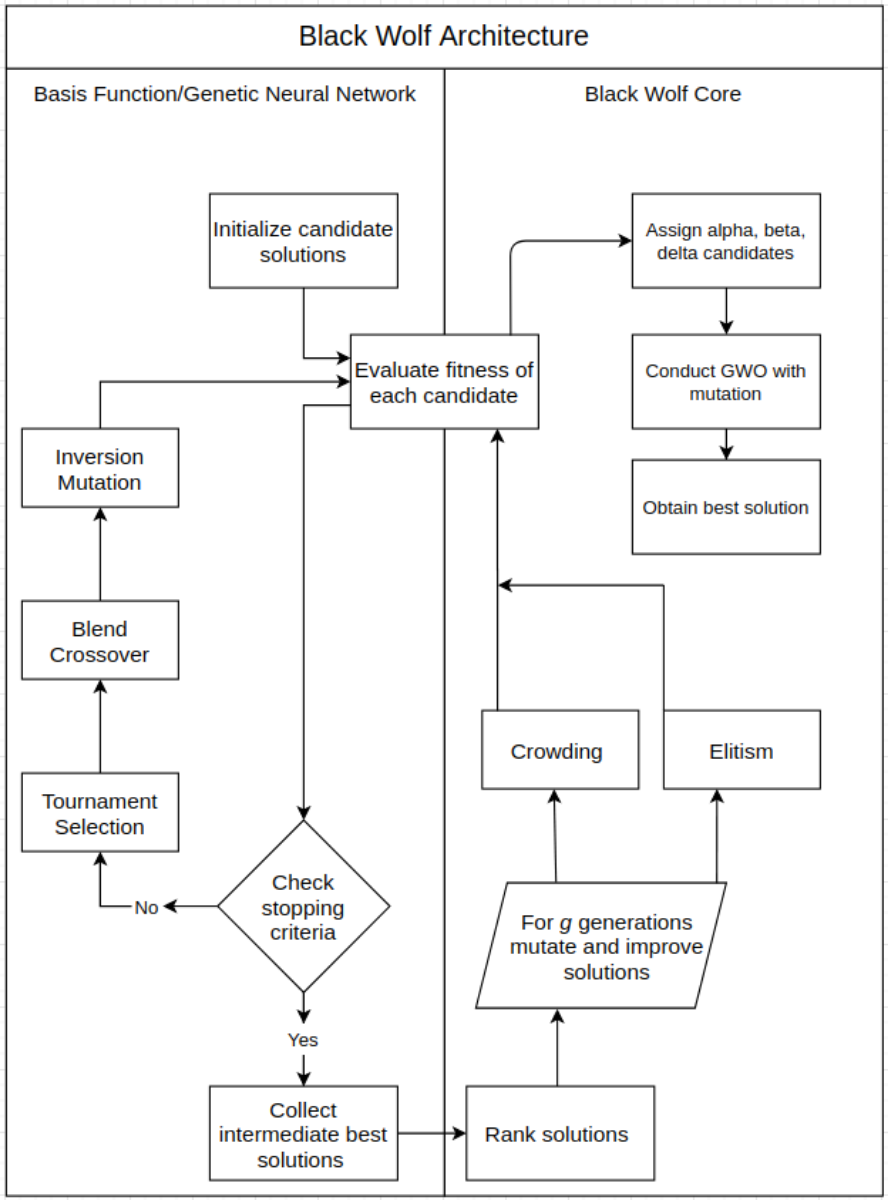
\includegraphics[height=9cm]{flow.png}
\caption{Overview of BWO}
\label{flow}
\end{figure}
To improve on the existing methodology, we had to break down the existing architecture into an atomic format and rebuild it with some added functionality. While neural networks are extremely sensitive to hyperparameter tuning, reconfiguring the hyperparameter set for each problem is too tedious and not feasible \cite{mat}. The secondary option of exhausting the entire search space was also discarded due to a lack of scalability and the sheer volume of computational resources required. We introduced GA into the mix, resulting in a Genetic Neural Networks (GNN), as illustrated in Algorithm $\ref{alg:gnn}$ and in Fig. $\ref{fgn}$. GNNs view hyperparameters as generational values instead of iterative values. The main difference between these two views lies in the updation pattern \cite{gnn}. While a traditional neural network updates the values based on a set rule, GNNs apply selection, crossover, and mutation to select those values over generations. 

In BWO, hyperparameters such as learning rate-dependent weights, momentum, dropout value, batch size, and initial estimates are selected from a pool of candidates by evaluating them against benchmark functions. The proposed genetic framework is developed upon the idea of a conventional grid search. GNN creates a grid and ranks various hyperparameter against each other. Other key details of selection, crossover, and mutation techniques are hashed out manually for optimal results. 

\begin{algorithm}[t]
\scriptsize
\caption{Genetic Neural Netowrk (GNN)}
\label{alg:gnn}
\begin{algorithmic}[1]
\STATE \textbf{Input:} Input vector $\vec{x}\textsubscript{i}$ and target vector $\vec{t\textsubscript{i}}$, population size $\textit{n}$, fitness function $\textit{f}$, number of generations $\textit{g}$
\FOR{Each  individual in $\textit{n}$}
\STATE Set selection technique as Tournament Selection
\STATE Set Blend crossover method 
\STATE Set Inversion mutation technique
\ENDFOR
\STATE Create class responsible for genetic grid search encapsulating all techniques specified
\STATE Deploy class over $\textit{g}$ and obtain hyperparameter configuration   
\STATE Call Algorithm $\ref{alg:nn}$ with the hyperparameter configuration and ($\vec{x}\textsubscript{i}$, $\vec{t\textsubscript{i}}$)
\end{algorithmic}
\end{algorithm}

\begin{figure}
\centering
\begin{subfigure}{5cm}
\centering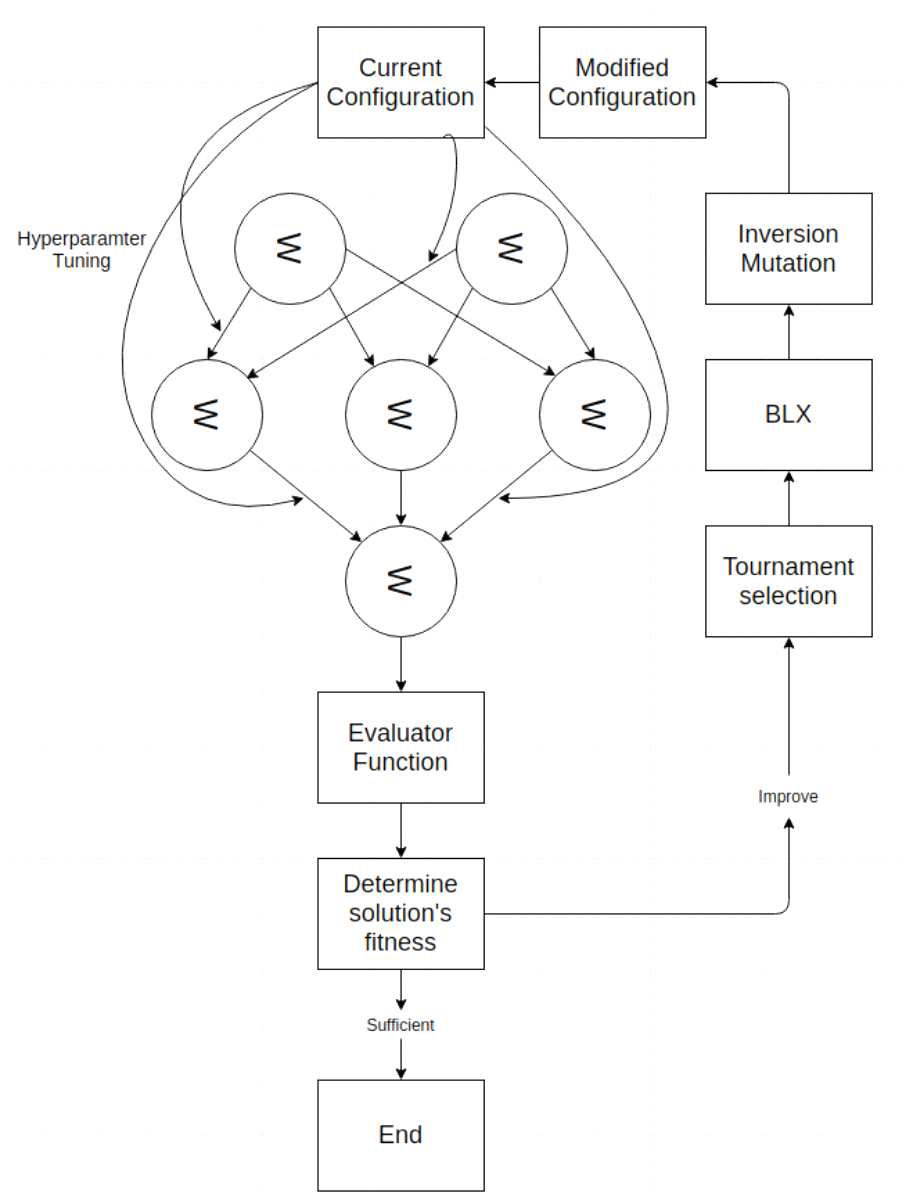
\includegraphics[height=8cm]{nn.png}
\end{subfigure}% 
\caption{Genetic Neural Network}
\label{fgn}
\end{figure}

The key steps used in Algorithm $\ref{alg:gnn}$ are:
\begin{itemize}
\item $\textbf{Tournament selection }$: 

Potential candidates compete against each other in a round-robin manner till the best candidates remain as depicted in Algorithm $\ref{alg:ts}$.
\begin{algorithm}[t]
\scriptsize
\caption{Tournament Selection}
\label{alg:ts}
\begin{algorithmic}[1]
\STATE \textbf{Input:} Candidate solution set $\textit{S}$, competition size $\textit{k}$,  tournament size $\textit{m}$ and fitness function $\textit{f}$
\FOR{Each round in $\textit{m}$}
\STATE Select $\textit{k}$ solutions from $\textit{S}$ without repetition and compare their fitness scores
\STATE Advance the qualified candidate
\ENDFOR
\end{algorithmic}
\end{algorithm}
% Selection techniques are applied at the begining of each generation, in order to select the best parents for that generation. This technique is a probabilistic one and since the fitness is directly correlated to getting selected for the next generation. In this techniques 2 or more candidates are selected from the pool of possible solutions and are made to compete in a tournament format. The candidate with the highest fitness score is selected as the victor. Note that the above fitness value score is not need as relativve scores are enough for elimination. 
\item 
$\textbf{Blend crossover(BLX)}$: 

Crossover methods take the selected candidates from the selection stages and perform crossover to generate the children of the parent solutions. These offsprings inherit the best characteristics of both its parents and hence is a better candidate solution. In BLX crossover, each offspring is randomly selected from an interval generated by its parents.
Equation $\ref{eq:blx}$ represents selection of offspring $O\textsubscript{i}$ from the range generated by parents $P\textsubscript{1,i}$ and $P\textsubscript{2,i}$ where $\textit{i}$ represents the $\textit{i\textsuperscript{th}}$ generation and $\alpha$ lies between 0 and 1.
%{\scriptsize
\begin{equation}
\label{eq:blx}
O\textsubscript{i} = [P\textsubscript{1,i} - \alpha(P\textsubscript{2,i} - P\textsubscript{1,i}), P\textsubscript{2,i} - \alpha(P\textsubscript{1,i} - P\textsubscript{2,i})] \scriptsize 
\end{equation}
%}%
\item $\textbf{Inversion mutation}$: 

Mutation is a probability based process which introduces a random change in a candidate solution. In inversion mutation, random hyperparameters $\textit{h}$ are selected from multiple candidates and swapped. This process is intended to introduce and promote diversity in the solutions. 

% The probability of a mutation occurring must be kept low to prevent degradation of the candidate's fitness. The mutation is necessary as it prevents any particular trait to dominate over others and hence promote diversity. As the name suggests inversion mutation a random subset of characteristics is selected and inverted.  
\end{itemize}
The process described in Algorithm $\ref{alg:gnn}$ is repeated for limited runs and a set of best possible network configurations are generated. Iterating over multiple generations and re-evaluating the network certainly has its drawbacks in the form of computational resource requirements and time taken. 
% As a visualization aid, genetic neural network process is dipicted in figure $\ref{fgn}$.

\subsection{BWO Core}
Black wolves follow a hierarchical pack order similar to grey wolves, which offers rank based solutions. GWO is formatted minimally, leaving a lot of room for improvement. The BWO Core improves on the existing optimizer by introducing a parallel niching along with mutation to engulf every local run into a global competition. 
\subsubsection{Niching Techniques}
At this stage, we extend the architecture to introduce niching which increases competition for the best resources. Difficult classification problems are computationally expensive and as a result parallel niching techniques are introduced. One of the most famous parallel niching techniques is crowding, depicted in Algorithm $\ref{alg:crowd}$ which introduces deterministic variation. 

\begin{algorithm}[t]
\scriptsize
\caption{Crowding}
\label{alg:crowd}
\begin{algorithmic}[1]
\STATE \textbf{Input:} Number of candidate solutions after genetic optimization $\textit{n}$, number of generations $\textit{g}$, fitness function $\textit{f}$
\FOR{Every generation in $\textit{g}$}
\WHILE{$\textit{n}$ is exhausted}
\STATE Randomly select 2 candidate solutions $n\textsubscript{1}$ and $n\textsubscript{2}$
\STATE Apply crossover and mutation to obtain solutions $m\textsubscript{1}$ and $m\textsubscript{2}$
\IF{$\delta($n\textsubscript{1}$, $m\textsubscript{1}$)$ + $\delta($n\textsubscript{2}$, $m\textsubscript{2}$)$ $\leq$ $\delta($n\textsubscript{1}$, $m\textsubscript{2}$)$ + $\delta($n\textsubscript{2}$, $m\textsubscript{1}$)$}
\IF{$\textit{f($m\textsubscript{1}$) $>$ f($n\textsubscript{1}$)}$}
\STATE Replace $n\textsubscript{1}$ with $m\textsubscript{1}$
\ENDIF
\IF{$\textit{f($m\textsubscript{2}$) $>$ f($n\textsubscript{2}$)}$}
\STATE Replace $n\textsubscript{2}$ with $m\textsubscript{2}$
\ENDIF
\ELSE
\IF{$\textit{f($m\textsubscript{2}$) $>$ f($n\textsubscript{1}$)}$}
\STATE Replace $n\textsubscript{1}$ with $m\textsubscript{2}$
\ENDIF
\IF{$\textit{f($m\textsubscript{1}$) $>$ f($n\textsubscript{2}$)}$}
\STATE Replace $n\textsubscript{2}$ with $m\textsubscript{1}$
\ENDIF
\ENDIF
\ENDWHILE
\ENDFOR
\end{algorithmic}
\end{algorithm}

\subsubsection{Elitism over generations}

Elitism counteracts the effects introduced by mutation and promotes survival of the Hall of Fame (HOF) members. HOF members represent the globally best solution. Elitism improves the performance by conserving the best fits encountered so far, decreasing the overall time taken by avoiding pitfalls in the genetic flow. This process is described in Algorithm $\ref{alg:eli}$.

\begin{algorithm}[t]
\scriptsize
\caption{Elistism}
\label{alg:eli}
\begin{algorithmic}[1]
\STATE \textbf{Input:} Candidate set $\textit{S}$, threshold value $\lambda$, and fitness function $\textit{f}$
\FOR{Each solution in $\textit{S}$}
\STATE Obtain fitness value for solution
\IF{Score exceeds $\lambda$}
\STATE Consider solution as elite
\ENDIF
\ENDFOR
\end{algorithmic}
\end{algorithm}

\subsubsection{Elemental Functionality of BWO}

At this stage, the best candidate solutions have been narrowed down through the pipeline. The candidates are now put through a GWO with a low mutation range for finally selecting the global optimum. The overall process can be understood with the following analogy. Consider a territorial distribution of wolf packs across a landmass with a single reward location. The genetically modified algorithm, along with niching and elitism, selects the best wolf from each pack. The final GWO stage makes the selected wolves compete against each other for the final treasure. This ensures global competition leading to increased assurance of guaranteed solution, increased parallelism, prevention of premature convergence, and automated hyperparameter tuning.  

% \begin{figure}[t]
% \centering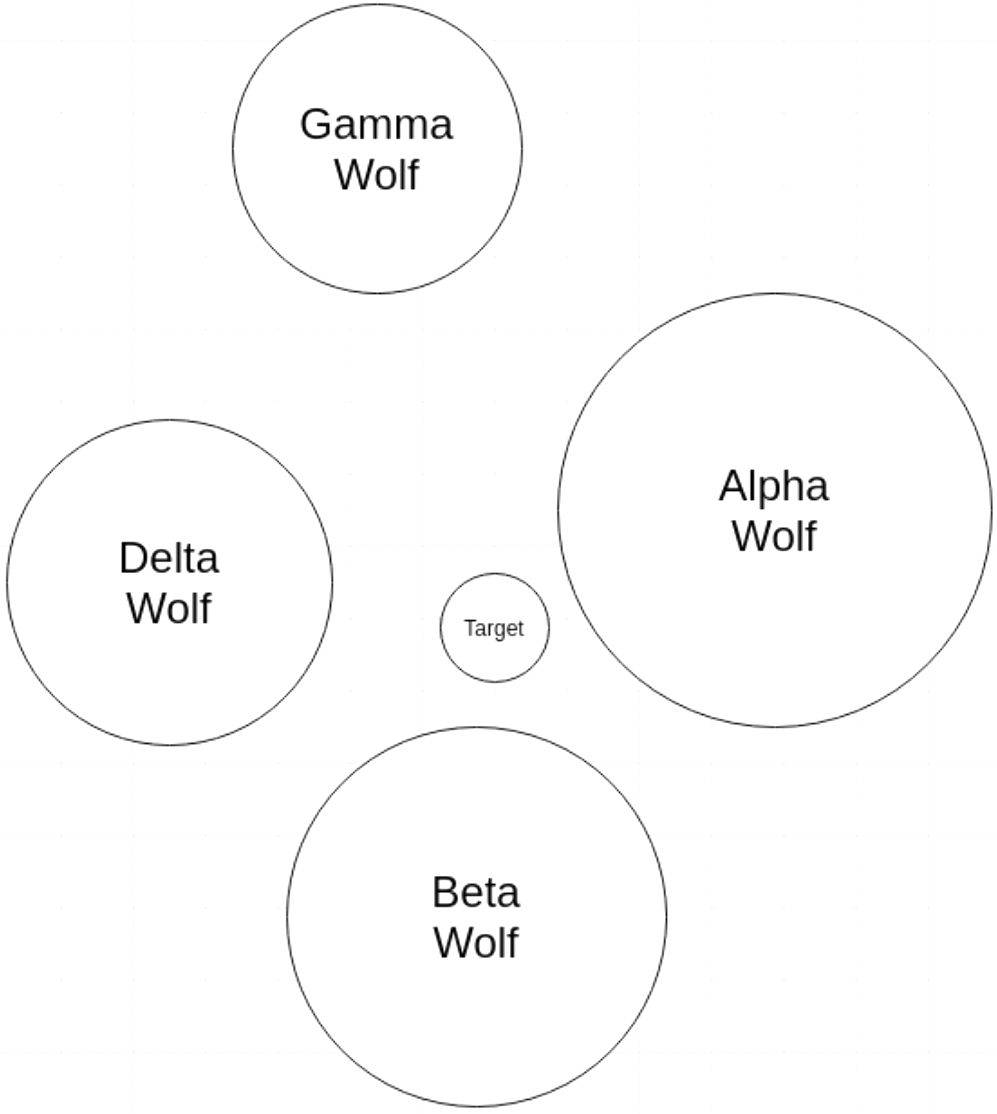
\includegraphics[width=4cm]{gwo.png}
% \caption{Final GWO step of BWO }
% \label{fig:gw}    
% \end{figure}

\subsection{Proof of Concept through Markov Chain Analysis}
In general, the offspring solutions produced by an EA are drawn from a fixed distribution. This process can be naturally modeled by a Markov chain (MC), which has been widely used to algorithmic analysis. A MC consists of a sequence of states $\epsilon\textsubscript{i}$ $\in$ {[0,$\infty$]}, where $\epsilon\textsubscript{i}$ depends on $\epsilon\textsubscript{i-1}$. Hence an entire MC can be described by its initial state $\epsilon\textsubscript{0}$ and transition conditions. 

Let $S\textsubscript{i}$ correspond to solution prompted by $\epsilon\textsubscript{i}$. Figure $\ref{fig:mc}$ display the Markov states along with their corresponding solution states. The aim of a MC analysis is to prove the convergence of the algorithm along with number of iterations need to reach the target state $S\textsuperscript{*}$. 

\begin{figure}[t]
\centering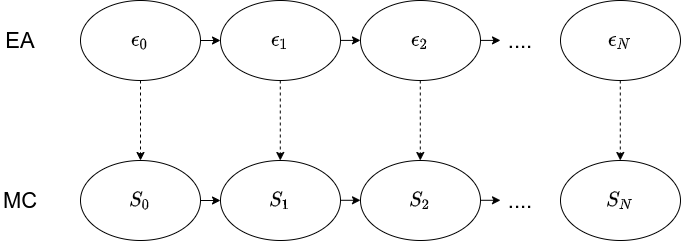
\includegraphics[width=7cm]{mc.png}
\caption{Markov Chain}
\label{fig:mc}    
\end{figure}

\theoremstyle{definition}
\begin{definition}[Convergence]
A Markov Chain $\epsilon$ having states sampled from distribution $\pi$ and target state $S\textsuperscript{*}$ is said to converge if,
\[ \lim_{i \to +\infty} \pi\textsubscript{i}(S\textsuperscript{*}) = 1\]
\end{definition}

\theoremstyle{definition}
\begin{definition}[Convergence Rate]

A Markov Chain $\epsilon$ having states sampled from distribution $\pi$ and target state $S\textsuperscript{*}$ is said to converge at a rate of $1 - \pi\textsubscript{i}(S\textsuperscript{*})$.
\end{definition}

Since BWO can be considered to be a specific implementation of EA, the proofs offered by Ding and Yu in \cite{he} with regard to asymptomatic convergence of EAs and their rate of convergence holds true for BWO too.  
\begin{table}[!t]
\caption{\textsc{Benchmark Functions}}
\label{tab:2}
\centering
\scalebox{0.7}
{
\begin{tabular}{| >{\arraybackslash}m{0.88in} | c | c | >{\arraybackslash}m{0.4in} | c | >{\arraybackslash}m{0.4in} |}
\hline
Function & ID & Formula & Modality & Range & Minimum Value \\
\hline
Sphere & F1 & $\sum_{i=1}^{n}(x\textsubscript{i}\textsuperscript{2})$ & Multi & [-100,100] & 0\\
Styblinski-Tang & F2 & $\frac{\sum_{i=1}^{n}x\textsubscript{i}\textsuperscript{4} - 16x\textsubscript{i}\textsuperscript{2} + 5x\textsubscript{i}}{2}$ & Multi & [-5,5] & -78.332\\
Three-hump Camel & F3 & $2x\textsuperscript{2} - 1.05x\textsuperscript{4} + \frac{x\textsuperscript{6}}{6} + xy + y\textsuperscript{3}$ & Multi & [-5,5] & 0\\
Matyas & F4 & $0.26(x\textsubscript{2} + y\textsubscript{2}) - 0.48xy$ & Uni & [-10,10] & 0\\
Brent & F5 & $(x + 10)\textsuperscript{2} + (y + 10)\textsuperscript{2} + e\textsuperscript{-(x\textsuperscript{2} + y\textsuperscript{2})}$ & Uni & [-10,10] & 0\\
Booth & F6 & $(x + 2y - 7)\textsuperscript{2} + (2x + y - 5)\textsuperscript{2}$ & Uni & [-10,10] & 0\\
\hline
\end{tabular}
}
\end{table}

\section{Experimental Setup and Result}

The entire BWO process is computationally expensive and time-consuming due to the repeated testing of the candidates. We could exploit the algorithmic level parallelism of the individual components of BWO and have accelerated them on HPC systems enabled with multiple GPUs. The results obtained from BWO have been compared with 5 other algorithms including GWO \cite{gwo}, Particle Swarm Optimization (PSO) \cite{pso}, Multiverse Optimization (MVO) \cite{mvo}, Cuckoo Search (CS) \cite{cs} and Bat Algorithm (BAT) \cite{bat}. 

\subsection{Data Description}

We have used both classical functions and real-world datasets to demonstrate BWO. This forked approach helps prove BWO's competence and it's use with real-world data. We have considered six benchmark functions to compare the performance of BWO with the other algorithms. We have further divided these functions into unimodal and multimodal functions to test the algorithms, as described in Table $\ref{tab:2}$. The artificial landscapes provided by these functions evaluate the general performance of an algorithm when presented with different scenarios. 

Data from a cohort study conducted in collaboration with a healthcare institute, with a cohort size of 100 oncology patients was collected. Based on the imaging, we could perform the Radiomics based feature extraction and preprocessing, which resulted in an initial set of radiomics features, on which we have applied the BWO and other methods. Data have also been collected from UCI Machine Learning repository for an extensive study with elaborated data sets, as listed in Table $\ref{tab:3}$. 

\begin{table}[t]
\caption{\textsc{Real-world Datsets}}
\label{tab:3}
\centering
\scalebox{0.75}
{
\begin{tabular}{ | c | c | c | c | c |}
\hline  
Dataset & ID & Source & Number of features & Number of Attributes\\
\hline
Oncological Cohort & D1 & HealthCare Institute& 97 & 16\\
Breast Cancer & D2 & UCI & 570 & 32\\
Parkinsons & D3 & UCI & 197 & 23\\
Liver Cancer& D4 & Kaggle & 345 & 7\\
\hline
\end{tabular}
}
\end{table}

\subsection{BWO Performance Model}

The BWO is modeled over a pipelined datapath consisting of $N_{Kernels}$ number of CUDA kernels, with adequate buffering. This section provides a performance model for the BWO on GPUs. The constants and definitions are listed in Table \ref{table2}.

\begin{table}[!t]
% increase table row padding
\renewcommand{\arraystretch}{1.3}
% if using array.sty, it might be a good idea to tweak the value of
% \extrarowheight as needed to properly center the text within the cells
\caption{\textsc{Constants and Definitions for BWO Performance Model}}
\label{table2}
\centering
\scalebox{0.8}
{
\begin{tabular}{| l | >{\arraybackslash}m{2.5in} |}
% \begin{tabular}{|l|l|}
\hline
\textbf{Symbols} & \textbf{Description}\\
\hline
$N_{Kernels}$ & No. of kernels in BWO \\
\hline
$IP_{BWO}$ & Total Application Data for BWO \\
\hline
$B_{Size}$ & Batch Size \\
\hline
$C_{Size}$ & Data chunk size transferred from CPU to GPU for one iteration of execution. \\
\hline
$N_{Batch}$ & Total number of batches over which GPU process $IP_{BWO}$ amount of data \\
\hline
$N\_C_k$ & No. of cycles for kernel k\\
\hline
$N\_B_k$ & No. of thread blocks per SM for kernel k\\
\hline
$N\_W_k$ & No. of warps per thread block for kernel k\\
\hline
$N\_T_{wgk}$ & No. of threads per thread block for kernel k\\
\hline
$N\_T_{wfk}$ & No. of threads per warp for kernel k\\
\hline
$N\_SM_k$ & No. of SMs required for kernel k\\
\hline
$N_{SM}$ & No. of SMs in the GPU\\
\hline
$N_{CSM}$ & No. of cores per SM in the GPU\\
\hline
$N\_Cores_k$ & No. of cores required for kernel k, and $N\_Cores_k = N\_SM_k \times N_{CSM}$\\
\hline
$P\_depth$ & Pipeline depth per core\\
\hline
$F_{GPU}$ & Clock rate of GPU\\
\hline
$N_{CORES}$ & Total no. of cores in GPU, and $N_{CORES} = N_{SM} \times N_{CSM}$\\
\hline
$N\_T_{Total}$ & Total no. of threads for kernel k, and $N\_T_{Total} \gg N_{CORES}$\\
\hline
$T_{Preprocessing}$ & CPU times for preprocessing batch input data\\
\hline
$T_{Postprocessing}$ & CPU times for postprocessing batch output data\\
\hline
$T_{CPU\_GPU}$ & Time spent to transfer buffer data from CPU to GPU\\
\hline
$T_{GPU\_CPU}$ & Time spent to transfer buffer data from GPU to CPU\\
\hline
$T_{kernel}$ & Time required for all the kernels to process the data in the current iteration\\
\hline
$N_{Batch}$ & Number of batches to cover the total application input data of $IP_{BWO}$\\
\hline
$N_{iter}$ & Total number of iterations required for all $N_{Batch}$ number of input batches\\
\hline
$N\_Ops_{BWO}$ & Total number of operations required across all batches of BWO runs\\
\hline
\end{tabular}
}
\end{table}


\par
The BWO Functional Model can be represented as: 

{\scriptsize
    \begin{equation}
    f(BWO) = f(\{k_1, k_2, \dots, k_{N_{Kernels}} \})
    \end{equation}
}%

% \subsubsection{BWO Batch Processing}
For BWO application data, $IP_{BWO}$, a single batch of input is scheduled for execution for a kernel $k$ over $N_{Tx\_Rx}$ iterations.

{\scriptsize
    \begin{equation}
    N_{Tx\_Rx} = \frac{B_{Size}}{C_{Size}} 
    \end{equation}
}%

{\scriptsize
    \begin{equation}
    N_{Batch} = \frac{IP_{BWO}}{C_{Size} \times N_{Tx\_Rx}}
    \end{equation}
}%

Following the parallel computing model, the total time required for a single iteration of inputs to exit the GPU can be given as:
{\scriptsize
    \begin{equation}
    \begin{split}
    T_{Gsi} = T_{Preprocessing} + \sum_{k = 1}^{N_{Kernels}}(T_{CPU\_GPU} + \\ T_{kernel} + T_{GPU\_CPU}) + T_{Postprocessing}
    \end{split}
    \end{equation}
}%

% 
% 
% where $T_{Preprocessing}$ and $T_{Postprocessing}$ are the CPU times for preprocessing and postprocessing the input and the output data respectively. $T_{CPU\_GPU}$ and $T_{GPU\_CPU}$ are the time spent in transfering data between CPU and GPU buffers. $T_{kernel}$ denotes the time required for all the kernels in the pipeline to process the data in the current iteration.

% \subsubsection{BWO Kernel Execution Time}
% The $N_{Kernels}$ number of kernels will run on the GPU in time, given by:


{\scriptsize
\begin{equation}
T_{BWO\_Kernel\_time} = \sum_{k = 1}^{N_{Kernels}}(T_{kernel_k})
\end{equation}
}%

% % The execution time for a single kernel $k$ is determined by the thread that takes the maximum number of cycles for execution on the GPU for that kernel. 
% {\scriptsize
% \begin{equation}
% N\_C_{Tmax} =  \stackbin[t = 1]{N\_T_{Total}}{max} (N\_C_{T_t})
% \end{equation}
% }%
% 
% % where $N\_C_{T_t}$ is decided by the extent of scheduling and latency hiding while the thread is running on the GPU. Extent of scheduling depends on the number of hardware units required for the thread and the the latency hiding is decided by the amount of private, local and global memory used for the thread, and the associated latency involved in transfer of data to and from the memory elements. 
% 
% Thus, the number of cycles required for executing kernel $k$ is given by:
% {\scriptsize
% \begin{equation}
% N\_C_k = \frac{N\_B_k \times N\_W_k \times N\_T_{wfk} \times N\_C_{Tmax}}{N_{CSM} \times P\_depth}
% \end{equation}
% }%

The time taken for executing kernel $k$ is represented by:
{\scriptsize
\begin{equation}\label{e15}
T\_Exec_k = \frac{N\_C_k}{F_{GPU}} 
\end{equation}
}%

% \subsubsection{BWO Kernel Runtime}
% The runtime of a kernel is a function of algorithmic complexity $\alpha$, memory model $\beta$ and GPU scheduling $\gamma$.  
% {\scriptsize
% \begin{equation}
% \alpha = f(B_{Size}, N_{Batch}, IP_{BWO}, L, N)
% \end{equation}
% }%
% 
% {\scriptsize
% \begin{equation}
% \beta = f(Occ_k, C_{Size}, Mem\_Latency)
% \end{equation}
% }%
% 
% {\scriptsize
% \begin{equation}
% \gamma = \frac{\gamma_{Occ} \times N\_B_{schd} \times N_{CSM}}{N\_B_k} 
% \end{equation}
% }%
% 

% Here, $N\_B_{schd}$ is the number of blocks which are in running state on the GPU. $\gamma_{Occ}$ is a lower limit of GPU occupancy while scheduling kernel $k$ and given by:
% \DeclarePairedDelimiter{\ceil}{\lceil}{\rceil}
% {\scriptsize
% \begin{equation}
% \gamma_{Occ} = \ceil*{\frac{N\_B_k}{N\_B_{schd} \times N_{CSM}}} 
% \end{equation}
% }%
% 
% We see that $\gamma_{Occ}$ indicates the minimum number of schedules required for covering the entire number of blocks requested to be run on GPU for kernel $k$. For any big data processing on GPU, $N\_B_k \gg N\_B_{schd}$.
% 
% {\scriptsize
% \begin{equation}
% N\_B_{schd} = f(\frac{Mem_k}{Mem_{SM}}, \frac{Reg_k}{Reg_{SM}}, \frac{N\_B_k}{N\_B_{SM}}, \frac{N\_T_{wgk}}{N\_T_{SM}})
% \end{equation}
% }%
% 
% where $Mem_k$, $Reg_k$, $N\_B_k$ and $N\_T_{wgk}$ denote the requirements for memory, registers, blocks and threads of the kernel $k$ respectively. $Mem_{SM}$, $Reg_{SM}$,  $N\_B_{SM}$ and $N\_T_{SM}$ represent the maximum values available per SM in the GPU. Thus, $N\_B_{schd}$ represents GPU occupancy for kernel $k$.

% Assuming that there are very large number of threads to be launched, the runtime dependencies of a kernel $k$ on the hardware resources, memory resources and scheduling factors can be expressed as:
% {\scriptsize
% \begin{equation}\label{e21}
% T_{kernel_k} \propto (\alpha \times \beta \times \gamma)
% \end{equation}
% }%
% 
% Again, for a kernel $k$ that requires $N\_Cores_k$ number of cores, the runtime can also be expressed as:
% {\scriptsize
% \begin{equation}\label{e22}
% T_{kernel_k} = f(\frac{N\_Ops}{N_{CORES}}, N\_Ops\_cp) 
% \end{equation}
% }%
% 
% Here, $N\_Ops$ represents the computational complexity of kernel $k$ i.e., the total number of computations performed by the kernel over multiple iterations and schedules. $N\_Ops\_cp$ represents the number of computations performed along the critical path of the kernel.
% \par
% Thus, combining (\ref{e15}), (\ref{e21}) and (\ref{e22}), the runtime for kernel $k$ can be expressed as:
% {\scriptsize
% \begin{equation}\label{e23}
% T_{kernel_k} \propto \bigg\{f(\frac{N\_Ops}{N_{CORES}}, N\_Ops\_cp) \times (\alpha \times \beta \times \gamma), T\_Exec_k\bigg\}
% \end{equation}
% }%

\subsubsection{BWO Multi-GPU Model}
% This section analyses the scalability of BWO on an HPC platform hosting multiple GPUs. 

% While distributing the data across multiple GPUs for parallel execution, we inherently parallelise the application itself across a set of $N_{GPU}$ GPUs. Thus, each GPU simultaneously handles an equal share of data, while following the GPU kernel runtime model described in the previous subsection. 
\par
The time taken by a single GPU to run $k$ kernels over $N_{Batch}$, is denoted by: 
{\scriptsize
\begin{equation}
T_{BWO\_Single} = \sum_{i=1}^{N_{iter}}(T_{Gsi})
\end{equation}
}%


\par
% Now, we can view a HPC platform as a distributed computing system on which BWO can run on $N_{GPU}$ number of GPUs by adopting data and task level parallelism. 

The average time taken for a single computation in BWO is given by:

{\scriptsize
\begin{equation}
t_{Single\_Op} = \frac{T_{BWO\_Single}}{N\_Ops_{BWO}}
\end{equation}
}%

The execution time of BWO on $N_{GPU}$ GPUs can now be modeled as:
\DeclarePairedDelimiter{\ceil}{\lceil}{\rceil}
{\scriptsize
\begin{equation}\label{e26}
T_{BWO\_Multi} \propto \bigg\{t_{Single\_Op} \times \ceil*{\frac{N\_Ops_{BWO}}{N_{GPU}}}\bigg\} 
\end{equation}
}%

% We measure the throughput of BWO as Million Maps Per Second (MMPS). The MMPS can be written as:
% 
% {\scriptsize
% \begin{equation}\label{e27}
% P_{BWO} \propto \bigg\{\frac{N\_Ops_{BWO}}{T_{BWO} \times 10^6}\bigg\}
% \end{equation}
% }%
% 
% Here, $T_{BWO}$ is the time taken in seconds, by a single GPU, which can be either $T_{BWO\_Single}$ in the case of a single GPU platform, or  ${T_{BWO\_Multi}}$ in case of multiple GPUs.

Thus, the performance and throughput of BWO has a scaling factor on HPC platforms with increase in the number of GPUs. 
% Thus we see that, the performance of BWO on a particular GPU platform is largely decided by the choice of the algorithm, the occupancy of the GPU, the amount private, local and global memory used and the number of cores put to use within the GPU hardware. The model also predicts that the performance and 

\subsection{Results}

All of the six algorithms were initially tested on the benchmark functions with 50 runs and the results are tabulated in Table $\ref{tab:4}$. The mean and the standard deviation values highlight the algorithm's ability to edge towards the global optima. 

\begin{table*}[t]
\caption{\textsc{Benchmark Results}}
\label{tab:4}
\centering
\scalebox{0.8}
{
\begin{tabular}{| c | c  c | c  c | c  c | c  c | c  c | c  c |}
\hline
{\textbf{Function}}&{\textbf{GWO}}&{}&{\textbf{PSO}}&{}&{\textbf{MVO}}&{}&{\textbf{CS}}&{}&{\textbf{BAT}}&{}&{\textbf{BWO}}&{}\\
\hline
{}&{\textbf{Mean}}&{\textbf{Std}}&{\textbf{Mean}}&{\textbf{Std}}&{\textbf{Mean}}&{\textbf{Std}}&{\textbf{Mean}}&{\textbf{Std}}&{\textbf{Mean}}&{\textbf{Std}}&{\textbf{Mean}}&{\textbf{Std}}\\
\hline
{F1}&{6.59E-07}&{6.34E-05}&{2.29E-06}&{6.94E-05}&{9.7E-06}&{3.87E-05}&{2.48E-08}&{3.67E-06}&{5.78E-06}&{4.90E-05}&{9.55E-07}&{5.67E06}\\
{F2}&{-79.6845}&{8.5612}&{-64.8977}&{19.1565}&{-70.3532}&{11.2847}&{-91.805}&{60.1456}&{-73.1563}&{5.8415}&{-75.4213}&{8.2577}\\
{F3}&{1.77E-18}&{8.78E-12}&{6.81E-15}&{1.79E-13}&{1.22E-15}&{3.5E-13}&{5.06E-11}&{7.67E-16}&{3.08E-16}&{4.04E-09}&{1.52E-15}&{1.72E-12}\\
{F4}&{6.89E-14}&{0.0051}&{4.62E-21}&{6.01E-5}&{8.84E-15}&{9.66E-4}&{8.42E-19}&{0.55}&{5.64E-15}&{0.0042}&{4.53E-25}&{6.32E-05}\\
{F5}&{2.58E-32}&{5.23E-07}&{2.43E-31}&{1.15E-04}&{7.23E-28}&{5.12E-03}&{1.52E-20}&{6.44E-05}&{3.81E-35}&{3.73E-03}&{3.59E-31}&{2.15E-05}\\
{F6}&{8.43E-21}&{0.0031}&{6.41E-11}&{6.84E-05}&{5.58E-10}&{0.0074}&{3.12E-16}&{0.041}&{4.62E-15}&{5.34E-06}&{7.12E-24}&{0.0048}\\
\hline
\end{tabular}
}
\end{table*}
\begin{table*}[!t]
\caption{\textsc{Dataset Metrics}}
\label{tab:5}
\centering
\scalebox{0.8}
{
\begin{tabular}{| c | c  c  c  c  c  c | c  c  c  c  c  c |}
\hline
{\textbf{Dataset}}&{}&{}&{\textbf{Accuracy}}&{}&{}&{}&{}&{}&{\textbf{Time Taken}}&{}&{}&{}\\
\hline
{}&{\textbf{GWO}}&{\textbf{PSO}}&{\textbf{MVO}}&{\textbf{CS}}&{\textbf{BAT}}&{\textbf{BWO}}&{\textbf{GWO}}&{\textbf{PSO}}&{\textbf{MVO}}&{\textbf{CS}}&{\textbf{BAT}}&{\textbf{BWO}}\\
\hline
{D1}&{77.54}&{71.24}&{74.67}&{68.15}&{76.48}&{95.84}&{33.12}&{27.15}&{14.85}&{18.74}&{35.18}&{1208.51}\\
{D2}&{96.85}&{85.49}&{91.74}&{84.51}&{84.15}&{93.87}&{107.15}&{114.23}&{102.87}&{212.78}&{113.76}&{4152.21}\\
{D3}&{91.45}&{88.74}&{94.51}&{95.15}&{92.15}&{89.17}&{76.12}&{65.56}&{43.85}&{68.35}&{49.23}&{2179.94}\\
{D4}&{84.21}&{91.51}&{94.25}&{91.64}&{87.34}&{92.57}&{51.24}&{51.74}&{49.67}&{99.84}&{54.18}&{1201.72}\\
\hline
% {}&{}&{}&{}&{}&{}&{}&{}&{}&{}&{}&{}&{}\\
% {}&{}&{}&{}&{}&{}&{}&{}&{}&{}&{}&{}&{}\\
% {}&{}&{}&{}&{}&{}&{}&{}&{}&{}&{}&{}&{}\\
% {}&{}&{}&{}&{}&{}&{}&{}&{}&{}&{}&{}&{}\\
% {}&{}&{}&{}&{}&{}&{}&{}&{}&{}&{}&{}&{}\\
\end{tabular}
}
\end{table*}
\begin{table}[t]
\caption{\textsc{GPU based metrics}}
\label{tab:6}
\centering
\scalebox{0.8}
{
\begin{tabular}{| l | >{\arraybackslash}m{0.57in} | >{\arraybackslash}m{0.57in} | >{\arraybackslash}m{0.57in}|}
\hline
{\textbf{GPU}}&{\textbf{Memory Utilization/GPU}}&{\textbf{Time Taken by BWO}}&{\textbf{Improvement Factor}}\\
\hline
{1X 940MX}&{95.501\%}&{236.574}&{34X}\\
\hline
{1X GeForce RTX 2080Ti}&{91.504\%}&{103.465}&{85X}\\
\hline
{2X GeForce RTX 2080Ti}&{70.633\%}&{64.727}&{175X}\\
\hline
{4X GeForce RTX 2080Ti}&{74.659\%}&{17.211}&{517X}\\
\hline
\end{tabular}
}
\end{table}


As we can observe, BWO outperforms the other algorithms in majority of the runs. It must also be noted that algorithms like BAT and GWO do perform comparatively better than BWO for benchmark functions F3 and F4. Same is observed for the real-world data-sets D2 and D3. BWO, whilst an extremely competitive algorithm, is still not immune to the No Free Lunch theorem. Moreover, the performance of any algorithm is restricted by the data fed into it. The reason as to why BAT and GWO outperform BWO in certain fields can be attributed to the inherent characteristics of the dataset. However, it must be noted that BWO provides great results at each run for each function in a general front. 

The existing framework for real-world oncological datasets consists of boosted decision trees and random forests, with average test accuracy levels ranginge from 75-87.5\%. The six algorithms are applied to these datasets and the results are formulated in Table $\ref{tab:5}$. As we can observe from the consolidated data, BWO outperforms its five competitors. This result was expected due to the strong base provided by GWO and the additional functionalities of genetic algorithms. However, it must also be noted that the time taken by BWO surpasses other algorithms by a factor of 20x-80x. 

\begin{figure}[t]
\centering\includegraphics[width=7cm]{1.png}
\caption{Profiling Graph}
\label{1}    
\end{figure}

\begin{figure}[t]
\centering\includegraphics[height=6cm]{2.png}
\caption{Profiling Values}
\label{2}    
\end{figure}

Exploiting the parallel nature of the algorithm, we ran the GNN component of BWO on accelerator platforms using GPUs. A list of the GPUs along with the accelerated BWO performance is shown in Table $\ref{tab:6}$. These performance results are built on an Intel i5-7200U CPU host. We can see that with a single NVIDIA GeForce RTX 2080Ti GPU, the performance scaled by a factor of 85x in comparison with the base CPU run. The non-linear performance scalability offered by BWO is evident with an acceleration of 517x using four NVIDIA GeForce RTX 2080Ti GPUs, following the theoretical predictions. The profiling values $\ref{2}$ and the corresponding graph $\ref{1}$ display the task distribution for one randomly chosen iteration. As presented, 92.9\% of the computation has been placed on the GPU. However it can be observed from table $\ref{tab:6}$ that as the number of GPUs increase, the memory utilization decrease as the inter-process communication time increases.  

\subsection{Conclusion and Future Work}

BWO provides a new Pareto front when it comes to the genre of computationally intelligent algorithms. It has the capability of "sniffing out" the global optimum in a constrained multi-objective landscape. By merging GA and SI, BWO obtains the best of both the worlds and uses them as a foundation for a novel architecture. 

For any future work, improvements can be made in the GPU memory utilization front as well as explore scalable acceleration. Launching multiple kernels and having complete control over thread deployment and utilization can augment performance. Moreover, the mutated GWO section of BWO can also be accelerated GPUs due to the parallel nature of the algorithm. The social hierarchy of the wolves can be extended to a general population and updated rules can be applied. 

% 
\begin{thebibliography}{00}
\bibitem{chankong} Chankong V., Haimes Y, Thadathil J., Zionts S. (1985), Multiple Criteria Optimization: A State of the Art Review, Decision Making with Multiple Objectives, Lecture Notes in Economics and Mathematical Systems 242, Edited by Y.Y. Haimes, V. Chankong, SpringerVerlag, 36.
\bibitem{fried}Friedrich T, Hebbinghaus N, Neumann F. Rigorous analyses of simple diversity mechanisms.In: Proceedings of genetic and evolutionary computation conference (GECCO), London, UK,July 2007. p. 1219–1225.
\bibitem{Osyczka}Osyczka, A: Multicriteria Optimization in Engineering, John Wiley, New York 1984.
\bibitem{gwo}Seyedali Mirjalili, Seyed Mohammad Mirjalili, Andrew Lewis. Grey Wolf Optimizer, Advances in Engineering Software 69 (2014) 46–61
\bibitem{bwolf} Apollonio, M., Mattioli, L, Scandura, M. Occurrence of black wolves in the Northern Apennines, Italy. Acta Theriol 49, 281-285 (2004).
\bibitem{wang}Wang J, Hu S (2019) An improved grey wolf optimizer based on differential evolution and elimination mechanism. Sci Rep 9:7181
\bibitem{jp}Jayapriya J, Arock M (2015) A parallel gwo technique for aligning multiple molecular sequences. In: 2015 International conference on advances in computing, communications and informatics (ICACCI). IEEE, pp 210–215
\bibitem{arora}Arora, S., Singh, H., Sharma, M., and Sharma, S., Anand P (2019) A New Hybrid Algorithm Based on Grey Wolf Optimization and Crow Search Algorithm for Unconstrained Function Optimization and Feature Selection. IEEE Access 7:26343–26361, 2019.
\bibitem{emary}Emary, E., Zawbaa, H. M, Hassanien, A. E. (2016). Binary grey wolf optimization approaches for feature selection. Neurocomputing, 172, 371–381.
\bibitem{singh}Singh N, Singh SB (2017) A modified mean grey wolf optimization approach for benchmark and biomedical problems. Evol Bioinform 13:1–28
\bibitem{mat}Matthias Feurer and Frank Hutter. Hyperparameter optimization. In Frank Hutter, Lars Kotthoff, and Joaquin Vanschoren, editors, AutoML: Methods, Sytems, Challenges, chapter 1, pages 3-37. Springer, December 2018.
\bibitem{gnn} Geoffrey MillerPeter M. ToddShailesh U. Hegde, Designing Neural Networks using Genetic Algorithms. Conference: Proceedings of the 3rd International Conference on Genetic Algorithms, George Mason University, Fairfax, Virginia, USA, June 1989
\bibitem{he}Ding L., Yu J. (2007) An Analysis About the Asymptotic Convergence of Evolutionary Algorithms. In: Wang Y., Cheung Y., Liu H. (eds) Computational Intelligence and Security. CIS 2006. Lecture Notes in Computer Science, vol 4456. Springer, Berlin, Heidelberg. https://doi.org/10.1007/978-3-540-74377-4_17
\bibitem{pso}J. Kennedy and R. Eberhart, "Particle swarm optimization," Proceedings of ICNN'95 - International Conference on Neural Networks, Perth, WA, Australia, 1995, pp. 1942-1948 vol.4, doi: 10.1109/ICNN.1995.488968.
\bibitem{mvo}H. Jia, X. Peng, W. Song, C. Lang, Z. Xing and K. Sun, "Hybrid Multiverse Optimization Algorithm With Gravitational Search Algorithm for Multithreshold Color Image Segmentation," in IEEE Access, vol. 7, pp. 44903-44927, 2019, doi: 10.1109/ACCESS.2019.2908653.
\bibitem{cs}C. Zefan and Y. Xiaodong, "Cuckoo search algorithm with deep search," 2017 3rd IEEE International Conference on Computer and Communications (ICCC), Chengdu, 2017, pp. 2241-2246, doi: 10.1109/CompComm.2017.8322934.
\bibitem{bat}D. Singh, R. Salgotra and U. Singh, "A novel modified bat algorithm for global optimization," 2017 International Conference on Innovations in Information, Embedded and Communication Systems (ICIIECS), Coimbatore, 2017, pp. 1-5, doi: 10.1109/ICIIECS.2017.8275904.
% \bibitem{b2} J. Clerk Maxwell, A Treatise on Electricity and Magnetism, 3rd ed., vol. 2. Oxford: Clarendon, 1892, pp.68--73.
% \bibitem{b3} I. S. Jacobs and C. P. Bean, ``Fine particles, thin films and exchange anisotropy,'' in Magnetism, vol. III, G. T. Rado and H. Suhl, Eds. New York: Academic, 1963, pp. 271--350.
% \bibitem{b4} K. Elissa, ``Title of paper if known,'' unpublished.
% \bibitem{b5} R. Nicole, ``Title of paper with only first word capitalized,'' J. Name Stand. Abbrev., in press.
% \bibitem{b6} Y. Yorozu, M. Hirano, K. Oka, and Y. Tagawa, ``Electron spectroscopy studies on magneto-optical media and plastic substrate interface,'' IEEE Transl. J. Magn. Japan, vol. 2, pp.    740--741, August 1987 [Digests 9th Annual Conf. Magnetics Japan, p. 301, 1982].
% \bibitem{b7} M. Young, The Technical Writer's Handbook. Mill Valley, CA: University Science, 1989.
\end{thebibliography}
% \vspace{12pt}
% \color{red}
% IEEE conference templates contain guidance text for composing and formatting conference papers. Please ensure that all template text is removed from your conference paper prior to submission to the conference. Failure to remove the template text from your paper may result in your paper not being published.

\end{document}
